\hyphenation{diffe-rent}
%%%%%%%%%%%%%%%%%%%%% Conclusions %%%%%%%%%%%%%%%%%
\chapter{Conclusions}
\label{ch:Conclusions}


This thesis is about the search for the double Higgs boson production mediated by the intermediate KK graviton and separately by the radion heavy resonances in the $bbZZ$ channel: one of the Higgs bosons decays to
two \Pqb quarks while the other decays to a pair of \PZ bosons which, in
turn, decay to a pair of neutrinos and a pair of electrons or muons. For this measurement we used 2016 data set with the integrated luminosity of $35.9\fbinv$ collected by the CMS experiment at the LHC in the proton-proton collisions at $\sqrt{s} = 13 \TeV$.

No statistically significant deviations from the SM predictions for
background processes have been observed, and 95\% upper confidence limits are reported for production cross section
of a KK graviton/radion times the branching fraction of the subsequent decay into an
HH system. The limits are derived for resonance masses in the 250 GeV to 1 TeV range.

This analysis became public in November 2018 ~\cite{CMS-PAS-HIG-17-032}. Now, according to the CMS Physics Coordination, CMS wants to see a combination of this analysis with the other $bbZZ$ analysis, which is focused on the 2 b jets, 2 leptons, 2 jets signature. 
Currents plans are to produce a paper for the Physical Review D (PRD), where we will report the best limits for all available $bbZZ$ channels. Of course, prior to the grand $bbZZ$ merge, each analysis combines the data from both dimuon and dielectron channels. The mass range to be covered in the combined measurement is also from 250 GeV to 1000 GeV.

%The sensitivity of the analysis is limited by statistical uncertainties, mainly by those associated to the normalizations of the major background components, \ie, the non-prompt lepton estimation, the scale uncertainties for \ttW and \ttZ, as well as by the uncertainties on the measured lepton efficiency. In the future refinements of the analysis,  the reduction of the systematic uncertainties will be a crucial aspect. In addition, increasing the amount of data analized will allows for a better background contraining, by increasing the number of bins in the final S/B ratio map, so that the dominance of backgrounds can be well stablished by regions and then be better constrained.       
 

\clearpage

\section*{CERN guide, S'Cool Lab teacher, Finance Club admin, Boxing Club coach}
\small

It has been a great pleasure to stay at CERN for four years. From the bottom of my heart I want to thank my adviser and my HEP group for such an opportunity. I have exploited all the possible areas of science, outreach, fun, and joy available at CERN. Well, almost all, and I know it is ridiculous, but I have not tried skiing...

I have been an official CERN guide, giving people tours to Antimatter Decelerator, ATLAS control room, The Low Energy Ion Ring complex, Proton Synchrotron, LHC control room, Data Centre, The SM18 facility (a world leading magnet test facility for testing magnets and instrumentation at low temperature and high currents), The Alpha Magnetic Spectrometer control room. Audience ranged from middle school kids to emeritus professors of science. 

Also I have been a teacher at the S'Cool Lab where high school students have a chance to come to CERN and build at this "cool" laboratory a real experimental setup and then conduct the experiment on their own. 

For more than a year I have been an administrative officer at the CERN Finance Club. I have been inviting top professionals from the finance and fintech companies to give talks at our club, I have started the quant group at the club, and have been the first to optimise our portfolio of stocks using Monte Carlo methods and also later with the minimisation technique. needless to say, that I learnt all those tools in High Energy Physics!

Last but not least, my friends from the CERN Powerlifting club introduced me to the Boxing Club. The rest is a history. I have been training people with the goal to improve their health. As a side effect, some picked up self-defence, others had fun and found themselves truly addicted to this combination of the hard work and laughter, and a few even became very much into the world of the intelligent boxing, which is about strategy and outworking the opponent.



\iftrue
\begin{figure}[h]
     \includegraphics[width=0.54\textwidth]{uni_of_geneva}
     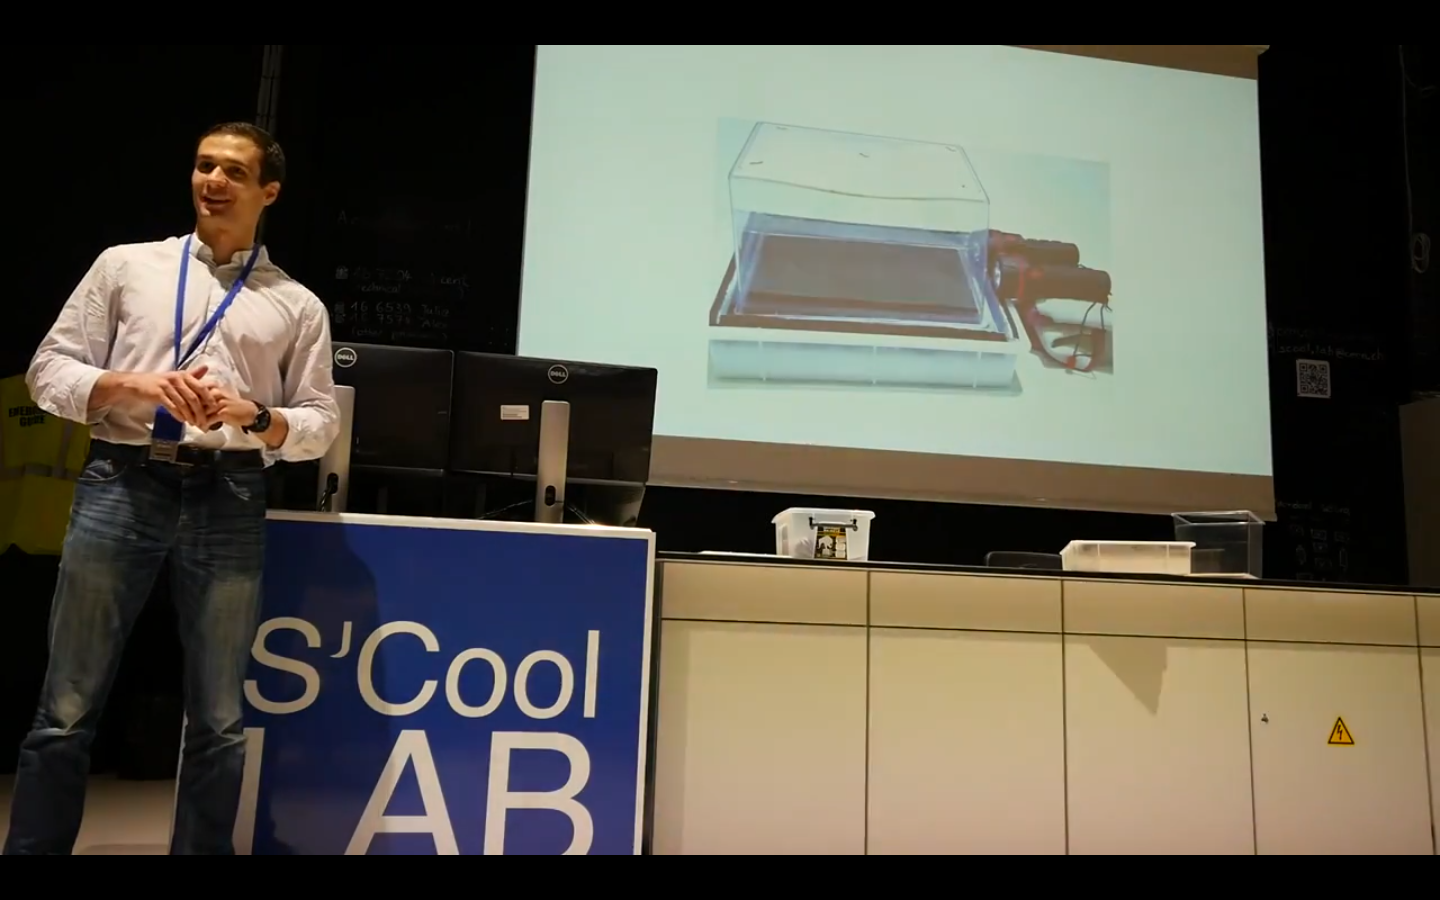
\includegraphics[width=0.54\textwidth]{scoollab2.png}\\
     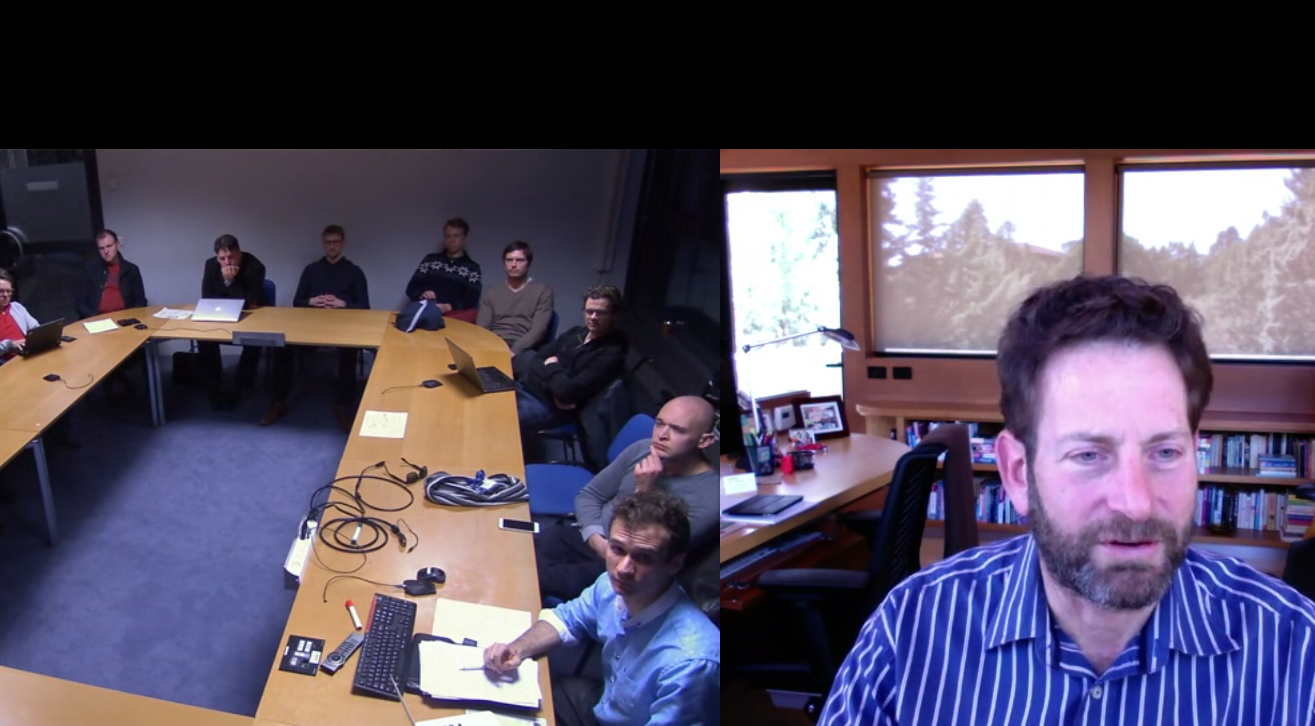
\includegraphics[width=0.54\textwidth]{finance1.png}
     \includegraphics[width=0.54\textwidth]{finance2.jpg}\\
     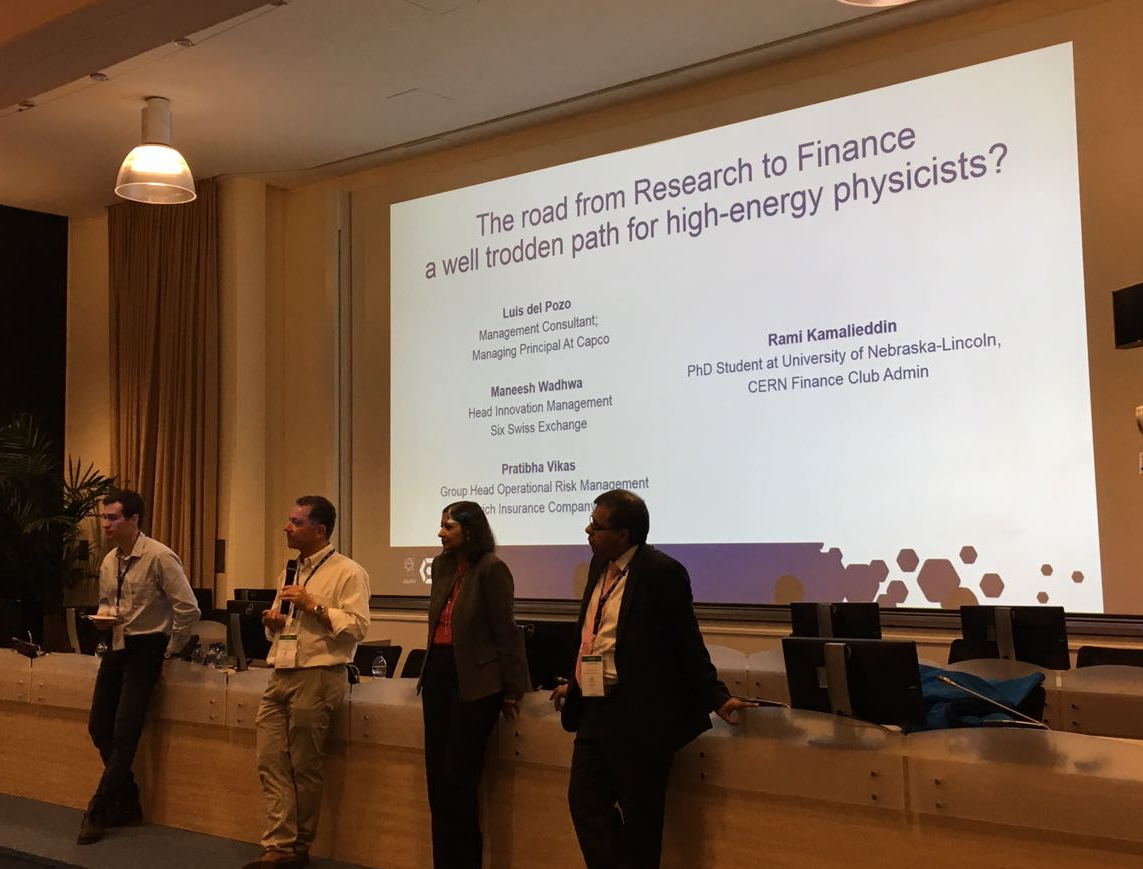
\includegraphics[width=0.54\textwidth]{finance3}
     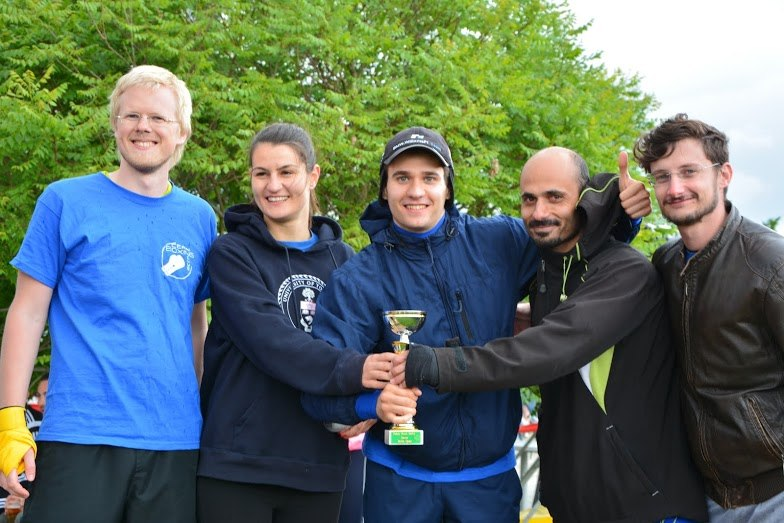
\includegraphics[width=0.54\textwidth]{boxing1.jpg}\\  
     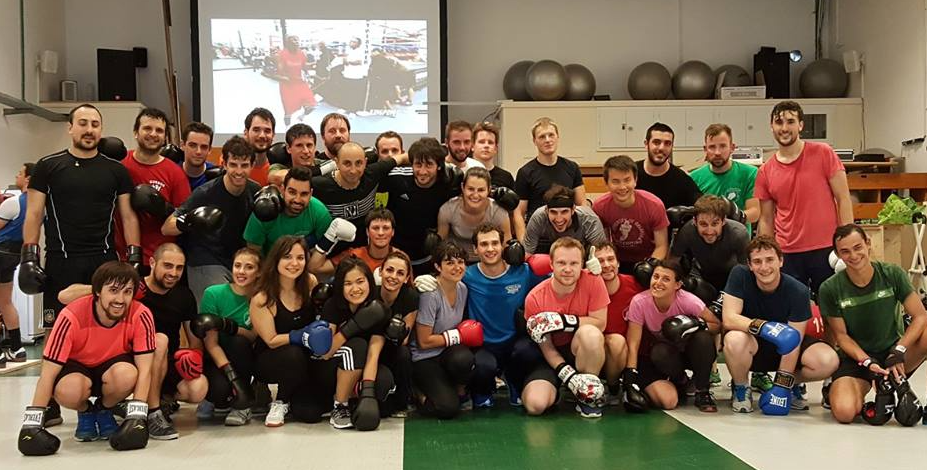
\includegraphics[width=0.54\textwidth]{boxing2}
     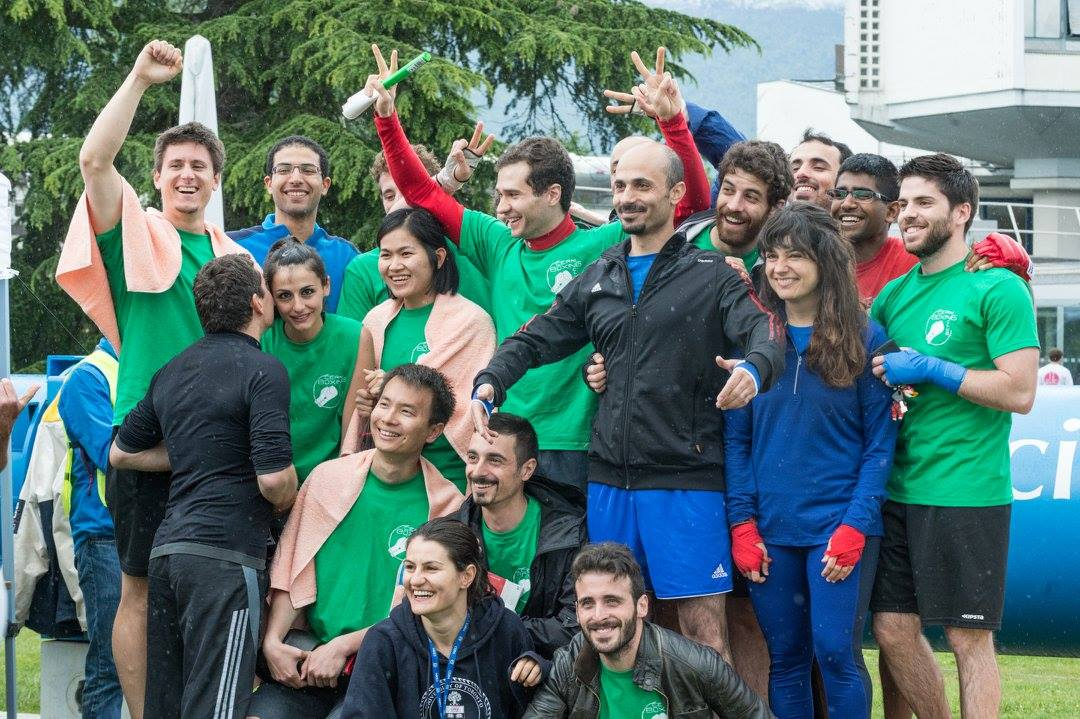
\includegraphics[width=0.54\textwidth]{boxing3.jpg}\\

   \end{figure}
\fi


